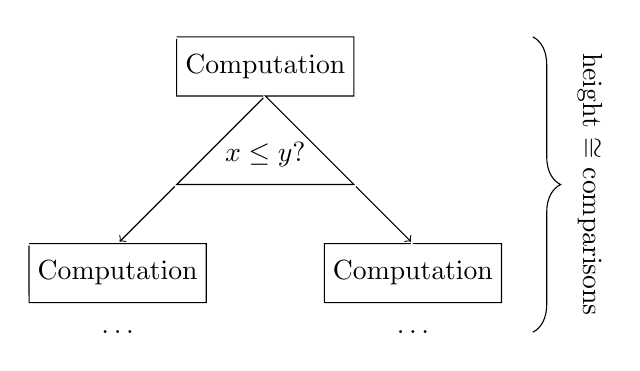
\begin{tikzpicture}[scale=0.75]
\usetikzlibrary{decorations.pathreplacing}

% \node [shape = rectangle, draw = black, minimum size = 2em] at (0,2) {Computation};
\node at (0,2) {Computation};
\node at (0,0.5) {$x \le y?$};
\node (v2) at (-2.5,-1.5) {Computation};
\node (v4) at (2.5,-1.5) {Computation};
% \draw (-1,.15) node (v1) {}  -- (0,1.65) -- (1,.15) node (v3) {} -- cycle;
\node at (-2.5,-2.5) {$\ldots$};
\node at (2.5,-2.5) {$\ldots$};
\draw [decorate,decoration={brace,mirror,amplitude=10,raise=-10}] (5,-2.5) -- (5,2.5) node {};
\node [rotate=-90] at (5.5,0) {height $\cong$ comparisons};
\draw (-1.5,2.5) node [inner sep=0] (v6) {} -- (1.5,2.5) node [inner sep = 0] (v9) {} -- (1.5,1.5) -- (0,1.5) node [inner sep=0] (v5) {} -- (1.5,0) node [inner sep=0] (cornerR) {} -- (-1.5,0) node [inner sep=0] (cornerL) {} -- (v5) -- (-1.5,1.5) -- (v6);
\draw (-4,-1) node [inner sep = 0] (v1) {} -- (-2.5,-1) node [inner sep=0] (v2) {} -- (-1,-1) -- (-1,-2) -- (-4,-2) -- (v1);

\draw (2.5,-1) node [inner sep=0] (v3) {} -- (4,-1) -- (4,-2) -- (1,-2) -- (1,-1) -- (v3);
\draw [->] (cornerL) edge (v2);
\draw [->] (cornerR) edge (v3);
\end{tikzpicture}